\modeCorrection

%%%% début de la page
\renewcommand{\thesection}{\textcolor{red}{Partie \Roman{section} -}}
\renewcommand{\thesubsection}{\textcolor{red}{\Roman{section}.\arabic{subsection}}}
\renewcommand{\thesubsubsection}{\textcolor{red}{\Roman{section}.\arabic{subsection}.\alph{subsubsection}}}

\setcounter{section}{0}
\setcounter{document}{0}
\sndEnTeteTPNeuf

\begin{center}
\begin{mdframed}[style=titr, leftmargin=60pt, rightmargin=60pt, innertopmargin=7pt, innerbottommargin=7pt, innerrightmargin=8pt, innerleftmargin=8pt]

\begin{center}
\large{\textbf{TP 9 : Phénomènes de réflexion en réfraction de la lumière
}}
\end{center}
\end{mdframed}
\end{center}

%\begin{tableauCompetences}
%    APP & Exploiter des explications orales pour rédiger un protocole & & & & \\
 %   \hline
  %  REA & Réaliser une série de mesures ; relever les résultats obtenus & & & & \\
   %  \hline 
    % REA & Utiliser une grandeur quotient pour déterminer le numérateur ou le dénominateur& & & & \\
     %\hline 
   % COM & Rendre compte de façon écrite & & & & \\
    %\hline
    %VAL & Analyser l’ensemble des résultats de façon critique  & & & &
%\end{tableauCompetences}


%%%% objectifs
\begin{tcolorbox}[colback=blue!5!white,colframe=blue!75!black,title=Objectifs de la séance :]
\begin{itemize}
    \item Mettre en évidence les phénomène de réflexion et de réfraction de la lumière ;
    \item Identifier une relation de proportionnalité ;
    \item Valider une loi en réalisant une série de mesures 
    \item Déterminer l'indice de réfraction d'un milieu ;
\end{itemize}
\end{tcolorbox}

%%%% Consignes
\begin{tcolorbox}[colback=red!5!white,colframe=red!75!black,title= Consignes :]
\begin{itemize}
    \item Faire attention au matériel lors de son utilisation ;
\end{itemize}
\end{tcolorbox}

%%%% contexte
\section{Mise en évidence expérimentale}
\begin{tcolorbox}[colback=orange!5!white,colframe=orange!75!black,title= Expérience introductive :]
Réalisons l'expérience suivante : on éclaire par une lumière laser une cuve initialement vide. Puis on remplit la cuve d'un mélange d'eau et d'une substance fluorescente permettant de visualiser la lumière laser. Voici les schémas de l'expérience avant et après remplissage de la cuve :
\begin{center}
    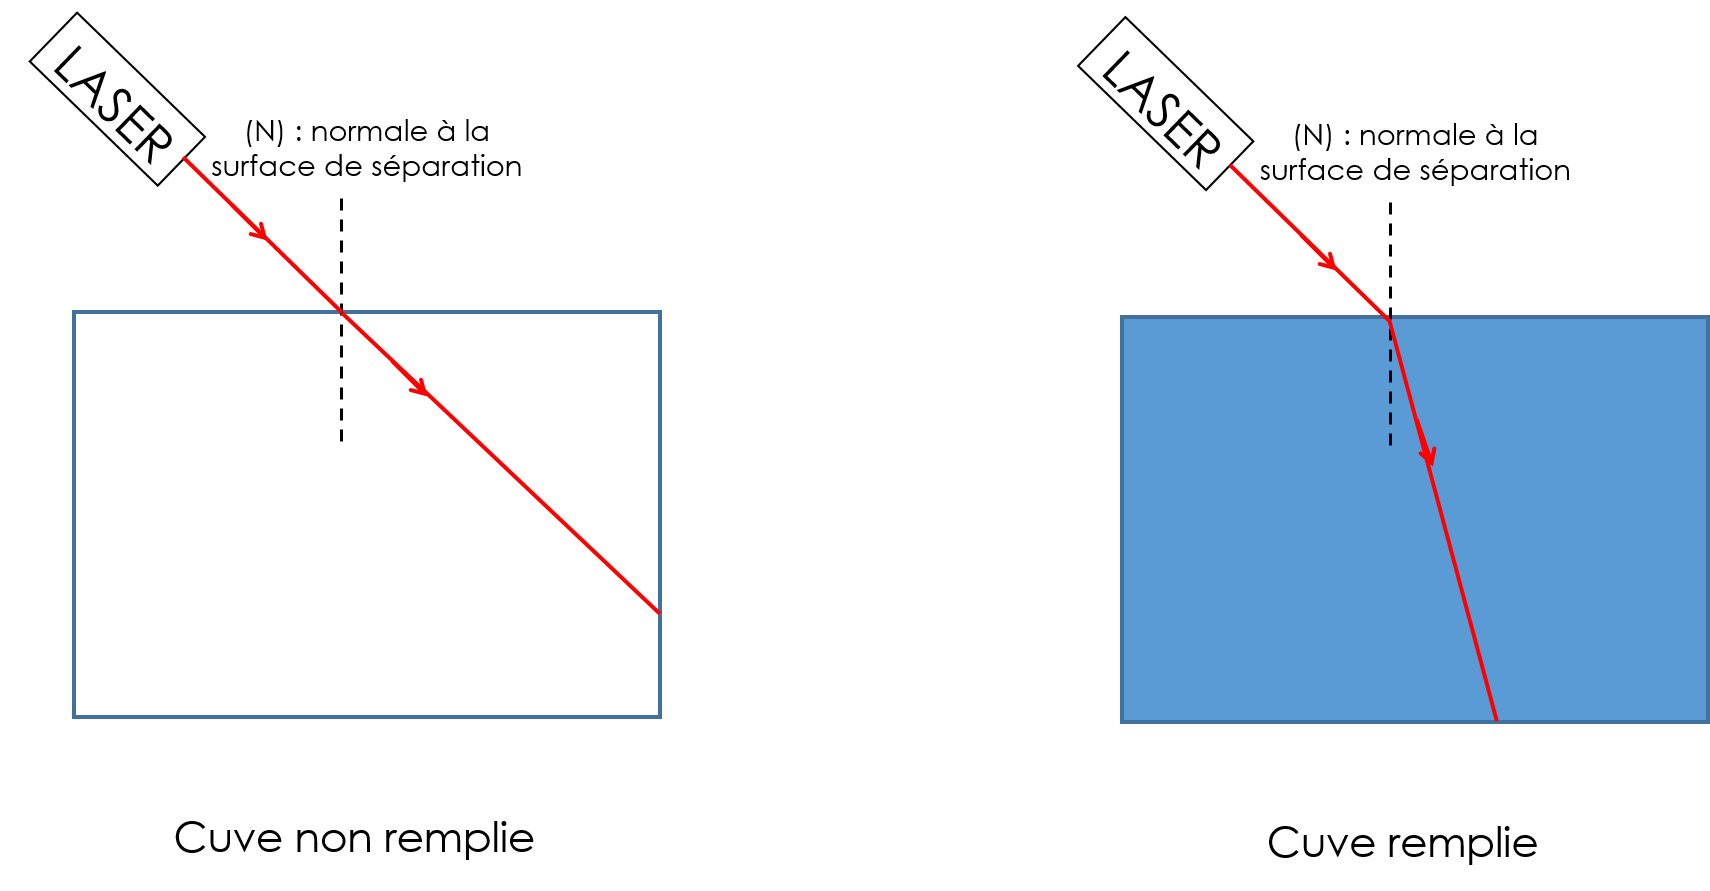
\includegraphics[scale=0.4]{Images/Experience_intro_correc.png}
\end{center}
\textbf{\underline{Observations :}}
\texteTrouMultiLignes{Lorsque la cuve est vide, la lumière provenant du laser se propage en ligne droite dans la cuve. En revanche, lorsque la cuve est remplie du mélange eau-fluorescéine, la lumière est déviée lors du passage air-mélange. La lumière se rapproche de la normale à l'interface.}{4}

\problematique{Peut-on relier les rayons refracté et réfléchi au rayon incident ? Peut-on mesurer un indice de réfraction d'un milieu ?}
\end{tcolorbox}


\begin{mdframed}[style=autreexo]
\textbf{\bsc{Liste du matériel}}
\begin{itemize}
    \item Une source de lumière collimatée avec son alimentation électrique ;
    \item Un demi-cylindre de plexiglas sur un disque gradué pivotant ;
    \item un ordinateur muni du logiciel tableau-grapheur ;
\end{itemize}
\end{mdframed}

%%%% documents

%%%%
\section{Lois de Snell-Descartes}
\begin{doc}{Quelques mots de vocabulaire}
\begin{center}
\vspace{-0.5cm}
     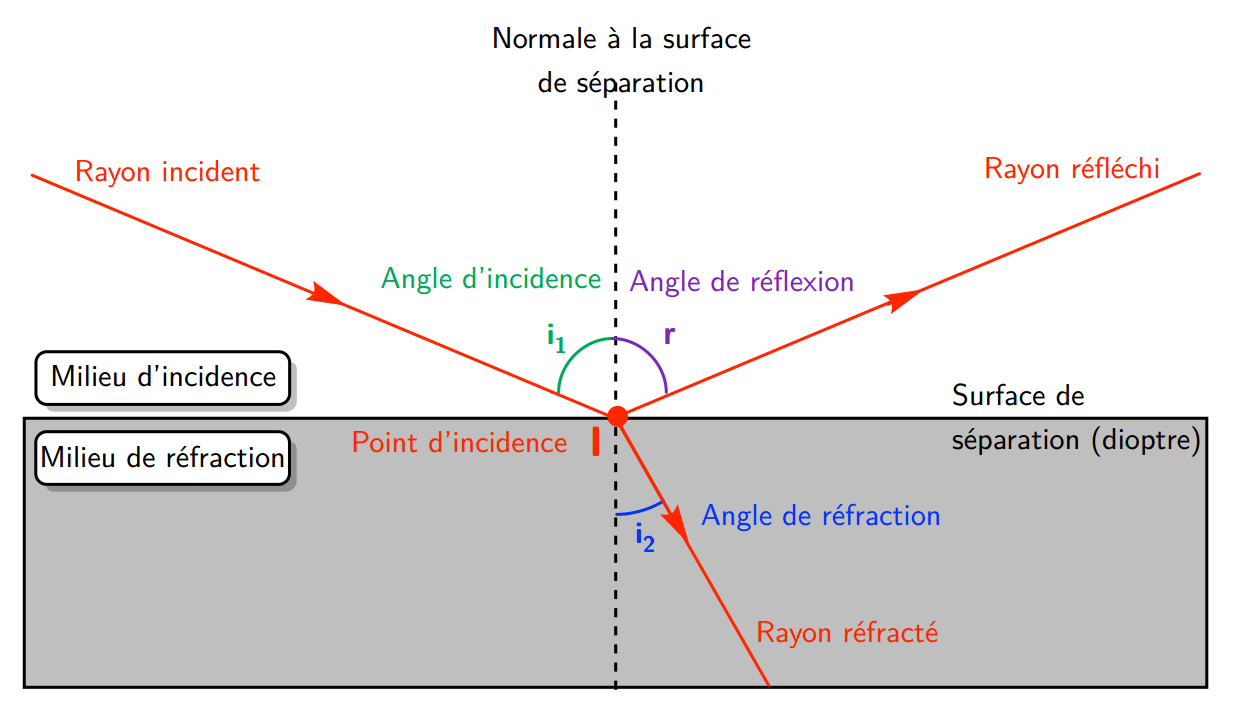
\includegraphics[scale=0.5]{Images/Figure_propagation.PNG}
\end{center}
\importantbox{Les angles d'incidence $i_1$, de reflexion $r$ et de réfraction $i_2$ sont toujours comptés à partir de la normale à la surface de séparation.}
\end{doc}

\subsection{Loi de Snell-Descartes pour la réflexion}
\begin{multicols}{2}
\question{Allumer la lampe et régler le zéro du disque gradué à l'aide des vis de réglage.}{Fais en classe.}{0}
\\
\question{Pour chaque valeur d'angle d'incidence $i_1$, mesurer l'angle de réflexion $r$ et compléter le tableau suivant :}{\begin{center}
    \begin{tabular}{|c|C{0.06}|C{0.06}|C{0.06}|C{0.06}|C{0.06}|C{0.06}|C{0.06}|C{0.06}|C{0.06}|}
        \hline
        $i_1$ (en $\degree$) & 0 & 5 & 10 & 15 & 20 & 30 & 35 & 40 & 45 \\
        \hline
        $r$ (en $\degree$) & 5 & 10 & 15 & 20 & 25 & 30 & 35 & 40 & 45\\
        \hline
    \end{tabular}
\end{center}}{0}
\begin{center}
    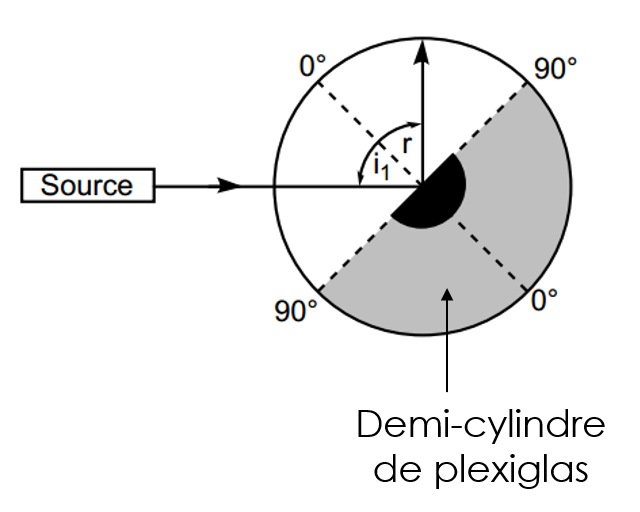
\includegraphics[width=0.4\textwidth]{Images/Schema_exp.PNG}
\end{center}
\end{multicols}

\begin{center}
    \begin{tabular}{|c|C{0.06}|C{0.06}|C{0.06}|C{0.06}|C{0.06}|C{0.06}|C{0.06}|C{0.06}|C{0.06}|}
        \hline
        $i_1$ (en $\degree$) & 0 & 5 & 10 & 15 & 20 & 30 & 35 & 40 & 45 \\
        \hline
        $r$ (en $\degree$) & & & & & & & & &\\
        \hline
    \end{tabular}
\end{center}
%\\
\begin{tcolorbox}[colback=red!5!white,colframe=red!75!black,title=\textbf{Loi de Snell-Descartes pour la réflexion : }]
\texteTrouMultiLignes{Les rayons incident et réfléchis sont tels que les angles d'incidence $i_1$ et de réflexion $r$ sont égaux : 
\begin{empheq}[box=\fbox]{equation*}
    i_1=r
\end{empheq}.}{2}
\end{tcolorbox}

\subsection{Loi de Snell-Descartes pour la réfraction}
\begin{center}
    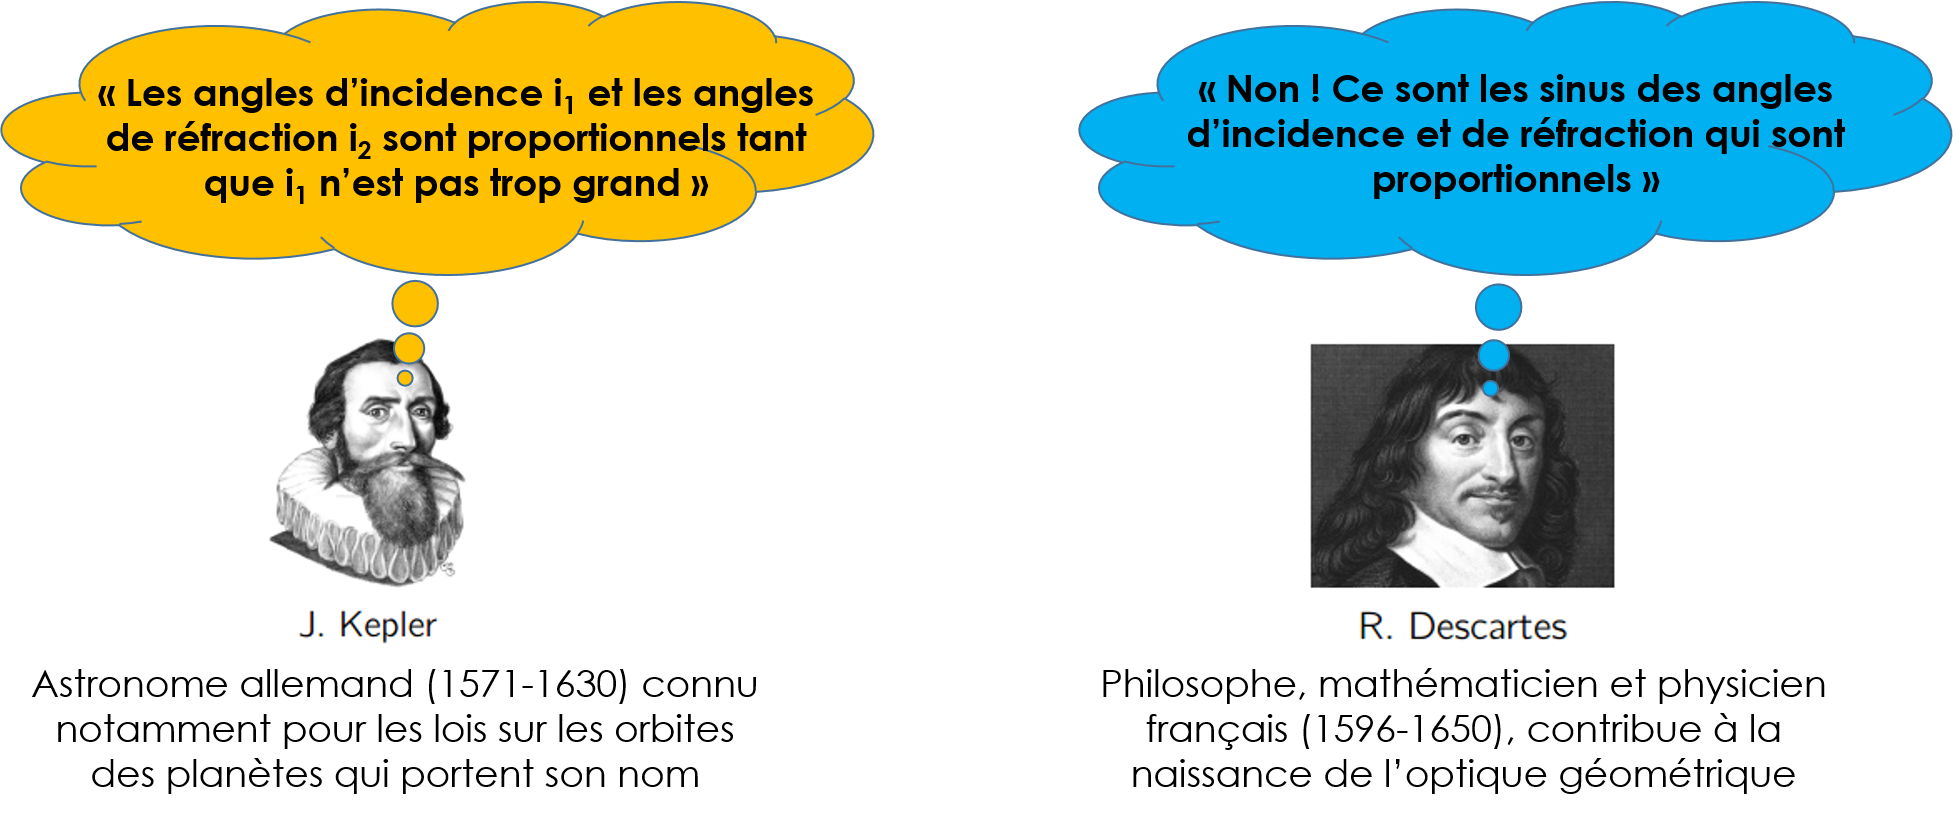
\includegraphics[scale=0.5]{Images/DescartesvsKepler.png}
\end{center}

\problematique{Lequel de ces deux scientifiques avait raison ?}
\subsubsection{Expérience}

\begin{multicols}{2}
\question{Allumer la lampe et régler le zéro du disque gradué sur le chemin du faisceau lumineux.}{Réalisé en classe.}{0}
\\
\question{Pour chaque valeur d'angle d'incidence $i_1$, mesurer l'angle de réfraction $i_2$ et compléter le tableau suivant (on ne prendra que 2 chiffres après la virgule pour le sinus) :}{~}{0}
\begin{center}
    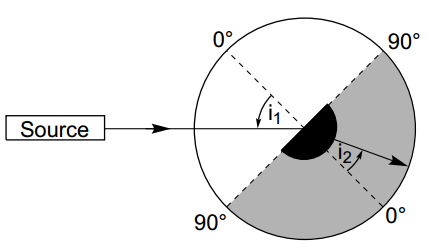
\includegraphics[width=0.4\textwidth]{Images/Schema_exp2.PNG}
\end{center}
\end{multicols}


\begin{center}
    \begin{tabular}{|C{0.1}|C{0.04}|C{0.04}|C{0.04}|C{0.04}|C{0.04}|C{0.04}|C{0.04}|C{0.04}|C{0.04}|C{0.04}|C{0.04}|C{0.04}|C{0.04}|C{0.04}|}
    \hline
        Angle $i_1$ (en $\degree$) & 0 & 5 & 10 & 15 & 20 & 25 & 30 & 35 & 40 & 45 & 50 & 60 & 70 & 80 \\
        \hline
        Angle $i_2$ (en $\degree$) & 0 & 3,5 & 7 & 10 & 13,5  & 16,5 & 20 & 23 & 25,5 & 28,5 & 31 & 36 & 39 & 41,5    \\
        \hline
        $\sin\left(i_1\right)$ & 0 & 0,09 & 0,17 & 0,26 & 0,34  & 0,42  & 0,50 & 0,57 & 0,64 & 0,71 & 0,77 & 0,87 & 0,94  & 0,98 \\
        \hline
        $\sin\left(i_2\right)$ & 0 & 0,06 & 0,12 & 0,17  & 0,23  & 0,28 & 0,34 & 0,39  & 0,43 & 0,48  & 0,52 & 0,58  & 0,63 & 0,66 \\
        \hline
        $\frac{i_1}{i_2}$ & non défini & 1,48 & 1,49 & 1,49 & 1,50 & 1,51 & 1,52 & 1,54 & 1,56 & 1,58 & 1,61 & 1,68 & 1,78 & 1,92  \\
        \hline
       $\frac{\sin\left(i_1\right)}{\sin\left(i_2\right)}$ & non defini & 1,6 & 1,5 & 1,5 & 1,5 & 1,5  & 1,5 &1,5  &1,5  &  1,5& 1,5 & 1,5  & 1,5 & 1,5  \\
        \hline
    \end{tabular}
\end{center}

\subsubsection{Exploitation des résultats}
\question{\`{A} partir des résultats expérimentaux, tracer sur le papier millimétré $i_2$ en fonction de $i_1$.}{\begin{center}
    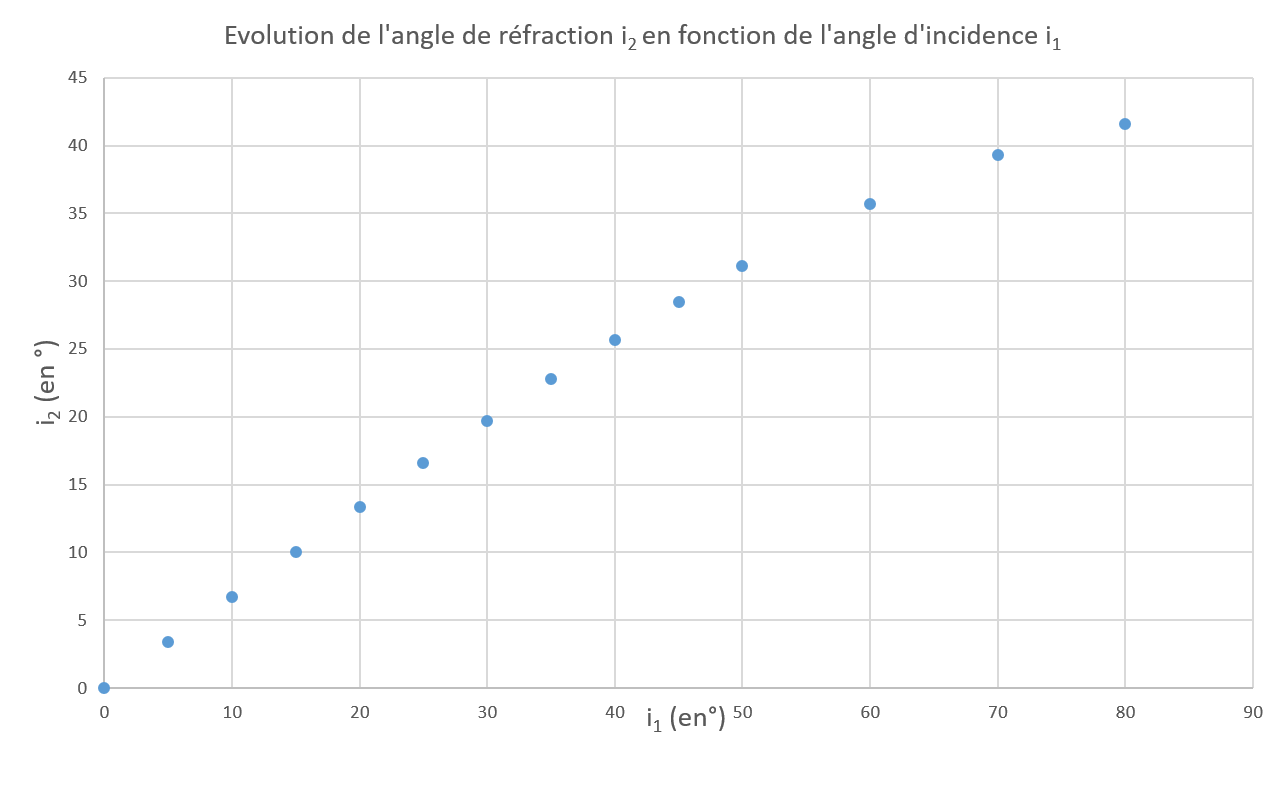
\includegraphics[scale=0.5]{Images/Refraction_i2vsi1.png}
\end{center}}{0}
%\\
\question{Johannes Kepler avait-il raison ?}{Oui à faible angle d'incidence, les angles $i_1$ et $i_2$ sont proportionnels comme on peut le voir sur le graphique ci-dessus.}{0}
\\
\question{Aller chercher le fichier \og TP9\_FeuilleCalculRefraction\_NomClasse\fg~sur l'ENT, dans l'espace documentaire de la classe.}{Fais en classe.}{0}
\\
\question{Reporter les valeurs de $i_1$ et de $i_2$ dans le tableau Excel. Convertir les angles $i_1$ et $i_2$ en radian (rad). Puis calculer les sinus de ces angles en utilisant la fonction SINUS() du tableur Excel.}{Fais en classe.}{0}
\\
\question{Tracer le graphique $\sin(i_2)=f(\sin(i_1))$ puis imprimez-le et coller-le sur votre compte-rendu.}{\begin{center}
    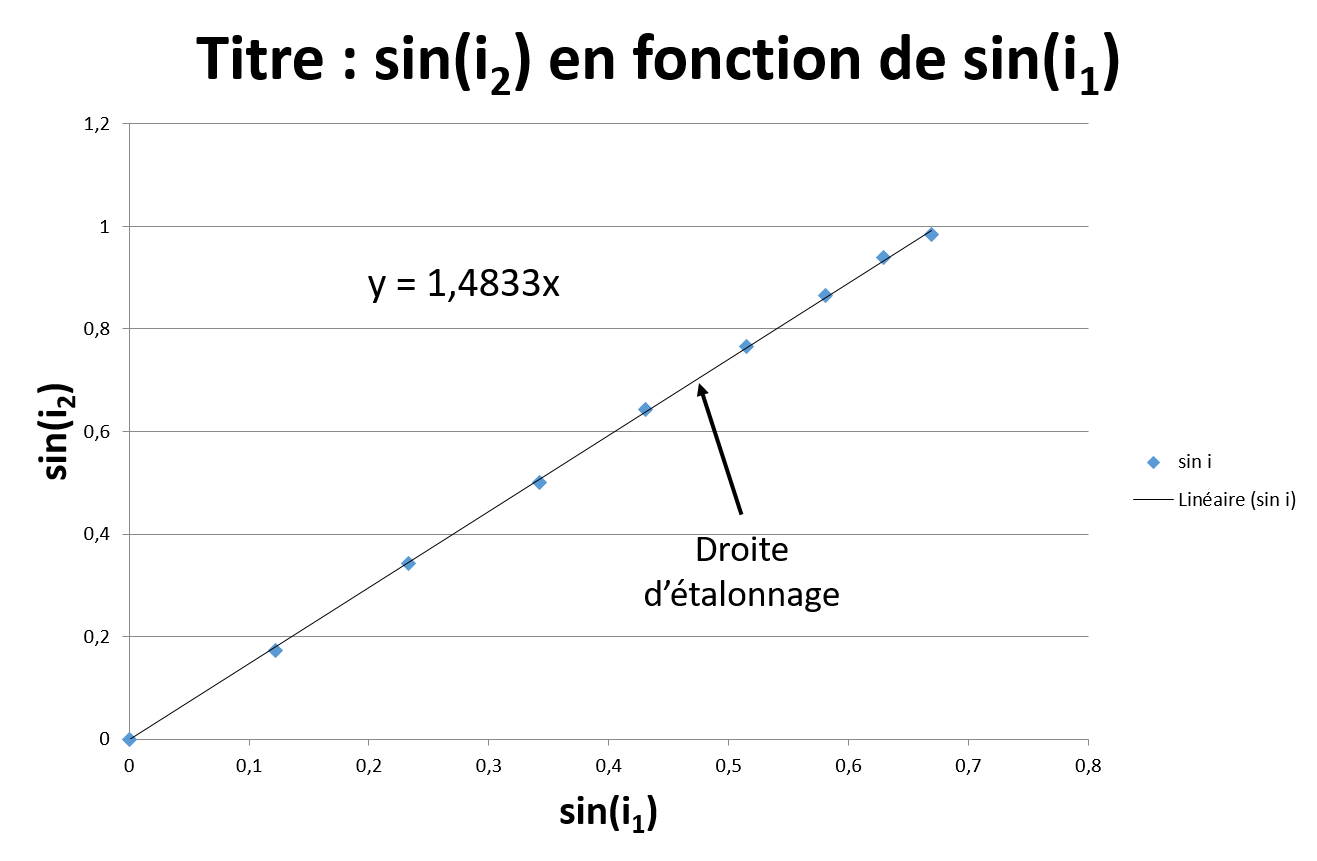
\includegraphics[scale=0.5]{Images/Refraction_resultats.png}
\end{center}}{0}
%\\
\question{En déduire qui de Kepler ou Descartes a énoncé la loi la plus valable. Justifier la réponse.}{C'est bien sûr Descartes car sa loi est valable pour n'importe quel angle d'incidence $i_1$, tandis que la loi énoncée par Kepler n'est valable que pour des petits angles d'incidence.}{0}
\\
On suppose que $\frac{\sin\left(i_2\right)}{\sin\left(i_1\right)} = \frac{n_2}{n_1}$ où $n_1$ et $n_2$ sont des nombres sans unités appelés \textcolor{red}{indices de réfraction}.\\
\question{En utilisant les fonctionnalités d’Excel (voir fiche méthode), déterminer une valeur expérimentale de $\frac{n_2}{n_1}$.}{A l'aide de l'équation de la droite d'étalonnage, on lit : $\frac{n_2}{n_1}=1,48$.}{0}

\begin{tcolorbox}[colback=red!5!white,colframe=red!75!black,title=\textbf{Loi de Snell-Descartes pour la réfraction : }]
\texteTrouMultiLignes{L'angle d'incidence $i_1$ est relié à l'angle de réfraction $i_2$ par la formule suivante :\begin{empheq}[box=\fbox]{equation*}
    n_1\sin\left(i_1\right)=n_2\sin\left(i_2\right)
\end{empheq}.}{2}
\end{tcolorbox}

\question{En sachant que $n_1=n_{air}=1$, déterminer la valeur de $n_2=n_{plexiglas}$.}{On détermine directement : 
\begin{equation*}
    n_{plexiglas} = 1,48\times n_{air} = 1,48
\end{equation*}
}{0}



%\newpage
%\papiermillimetre